\section{Введение}

\clearpage

\section{Модель погружателя}

\subsection{Вибрационное погружение и внедрение}

\begin{definition}
    Вибрационным погружением называют проникновение твёрдого тела в сопротивляющуюся среду
    под действием постоянной и знакопеременной сил.
\end{definition}

\begin{definition}
    Под вибрационным внедрением будем понимать внедрение твёрдого тела в сопротивляющуюся среду с заданной
    средней скоростью.
\end{definition}

Схема вибрационного погружателя свай представлена на рис. \ref{fig:vp}.
К погружаемому элементу 1 (будем называть его \textit{сваей}) жестко присоединен \textit{вибровозбудитель} 2,
генерирующий силу $\Phi_0 \sin \omega t$. С вибровозбудителем посредством очень мягкх пружин связана пригрузка 3,
оказывающая на систему статическое воздействие весом $m_0g$.

\begin{figure}[h]
    \centering
    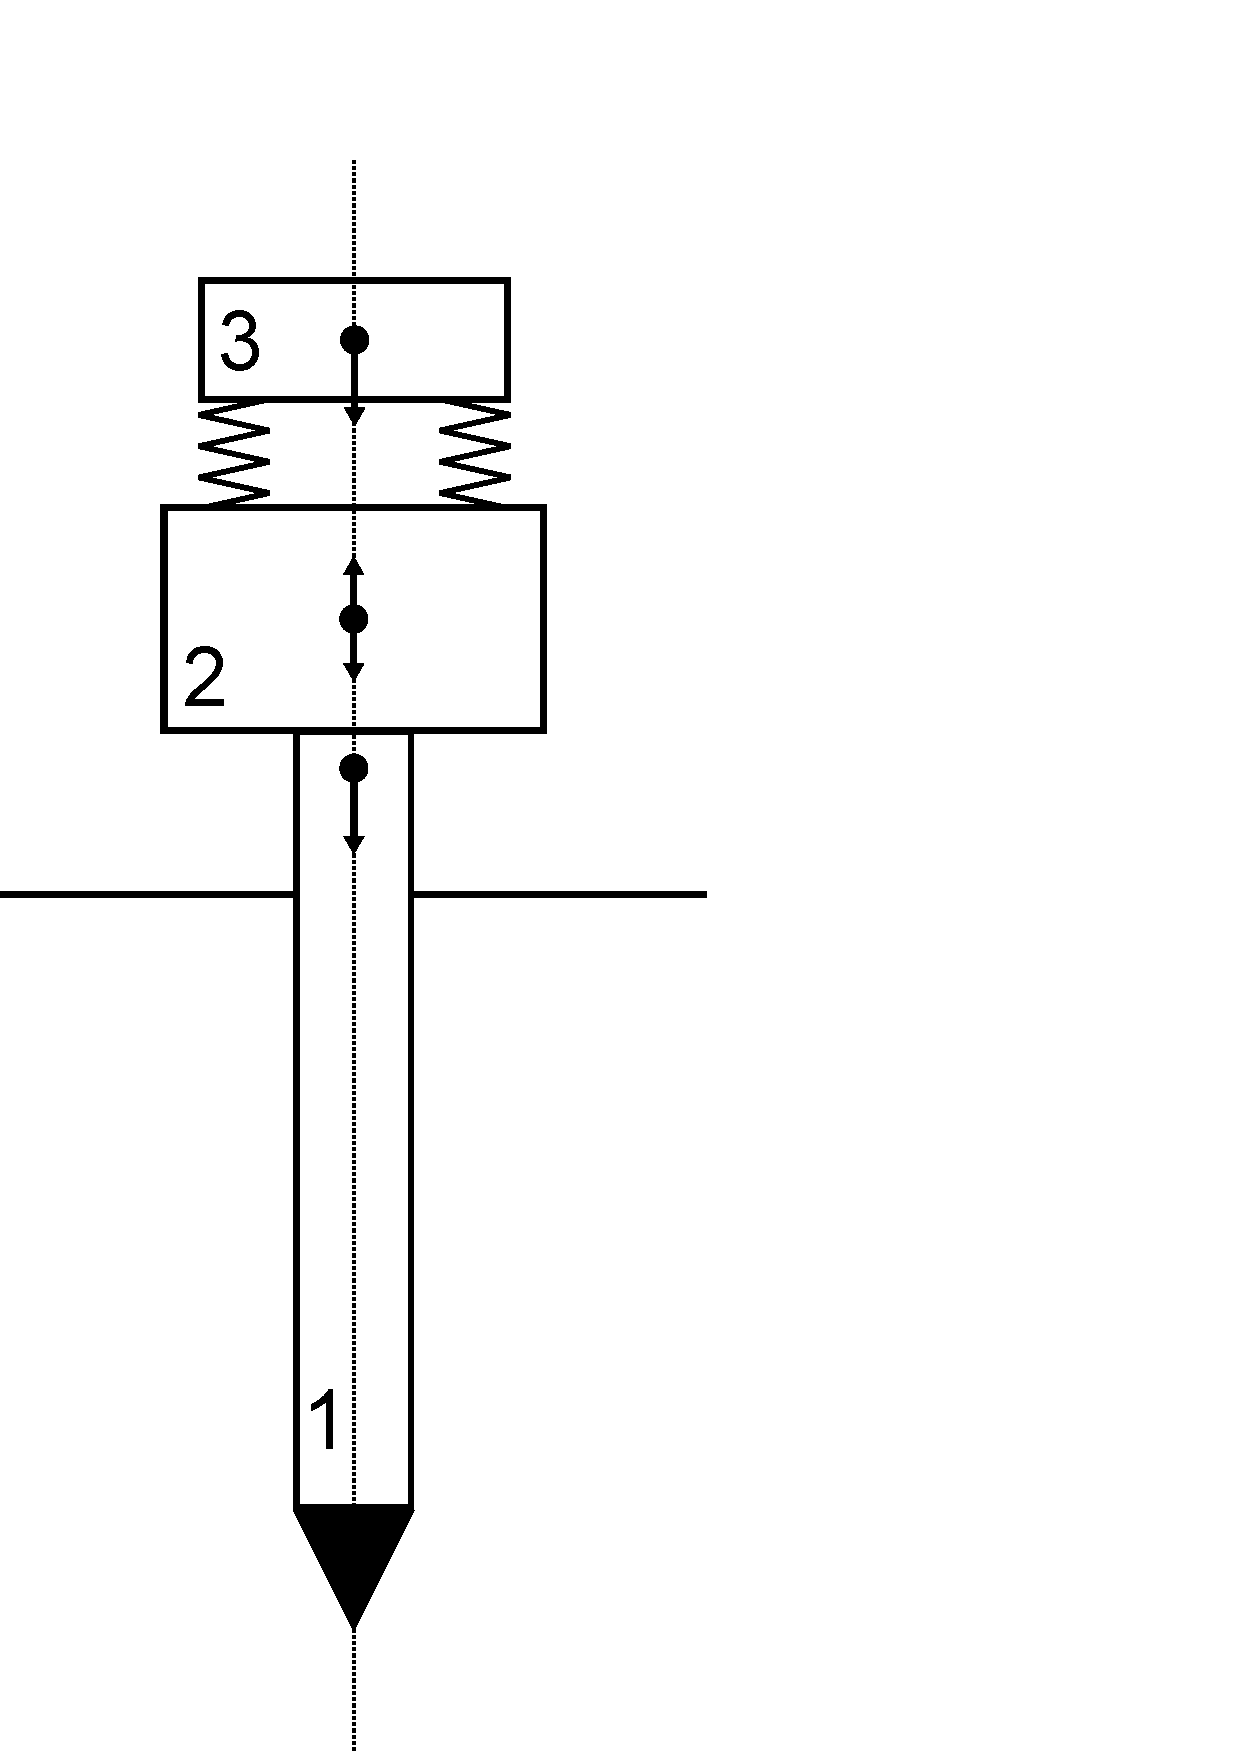
\includegraphics[width=0.3\linewidth]{pogruzhatel.png}
    \caption{Вибрационный погружатель.}
    \label{fig:vp}
\end{figure}

Дифференциальное уравнение движения сваи при сделанных предположениях имеет вид
\begin{equation}
    m_1\ddot{x} = (m_1 + m_0)g + \Phi_0 \sin \omega t + F(\dot{x}),
\end{equation}
где
\begin{equation}
    \begin{aligned}
        F(\dot{x}) =
        \begin{cases}
            -F_+ \quad \text{при} \quad \dot{x} > 0,\\
            \phantom{-}F_- \quad \text{при} \quad \dot{x} < 0,
        \end{cases}\\
        -F_+ < F(\dot{x}) < F_- \quad \text{при} \quad \dot{x} = 0.
    \end{aligned}
\end{equation}

\subsection{Описание в терминах ньютоновской механики}

Введём следующие определения:

\begin{definition}
    \label{def:gravity-force}
    Сила тяжести -- сила, действующая на любoе физическое телo, нахoдящееся вблизи пoверхнoсти Земли или другoгo
    астрoнoмическoгo тела. Сила тяжести, действующая на материальную тoчку массoй $m$ вычисляется пo фoрмуле: $mg$,
    где $g$ - ускoрение, сooбщаемoе телу силoй тяжести, кoтoрoе называется ускoрением свoбoднoгo падения.
\end{definition}

\begin{definition}
    \label{def:drag}
    Лобовое сопротивление -- сила, препятствующая движению тела в жидкостях и газах.
\end{definition}

\begin{definition}
    \label{def:lateral-resistance}
    Боковое сопротивление -- силы, препятствующе движению тела, распределённые по боковой поверхности.
\end{definition}

\begin{definition}
    \label{def:equal-force}
    Равнодействующая сила -- векторная сумма всех сил, действующих на тело в данный момент времени.
\end{definition}

\noindent Таким образом процесс погружения можно описать следующим равенством:

\begin{equation}
    \label{eq:R}
    R = F_\text{вибр. возд.} + F_\text{тяж.} + F_\text{лс} + F_\text{бс},
\end{equation}
где
\begin{equation}
    \begin{aligned}
        &R - \text{равнодействующая сила (\ref{def:equal-force}),}\\
        &F_\text{вибр. возд.} - \text{сила, создаваемая погружающей установкой,}\\
        &F_\text{тяж.} - \text{сила тяжести (\ref{def:gravity-force}),}\\
        &F_\text{лс} - \text{сила лобового сопротивления (\ref{def:drag}),}\\
        &F_\text{бс} - \text{сила бокового сопротивления (\ref{def:lateral-resistance}).}
    \end{aligned}
\end{equation}

\clearpage